\newpage

\section{Theory}

This section will be a trivially way of explaining how the YOLO algorithm work. It will also contain explanations of how the different parts of the algorithm works.

\subsection{Convolutional Neural Network}
Convolutional Neural Networks (CNN) is a part of the backbone structure of most object recognition software, as well as YOLO. Therefor it is important to understand how the recognition part of the algorithm works

A CNN consists of an input layer and an output layer. In between there are multiple hidden layers, who is not of any importance, exept the CNN it self. In the hidden layers is where the processings are happening. In the YOLO algorithm, the hidden layers consists of convolutional layers, max pool layers and fully connective layers \cite{YOLO}.


\subsubsection{Convolutional layers}
Applies learnable convolutional filters to the input data. YOLO utilises as many as 24 convolutional layers. Each layer add their own feature to the image. The convolutions runs spatialy trough the input image. Sliding in height, width and trough the different layers. The convolution net could be divided into 10x10x3 pixels (px). This meaning an image of 100x100x3 px need 100 convolution when going trough one small image. 

The important information that comes from the convolutional filter contains details of the image, how pixels are arrange in spatial and what object is in those pixels \cite{SF_ConvNet}.

\begin{figure}%
    \centering
        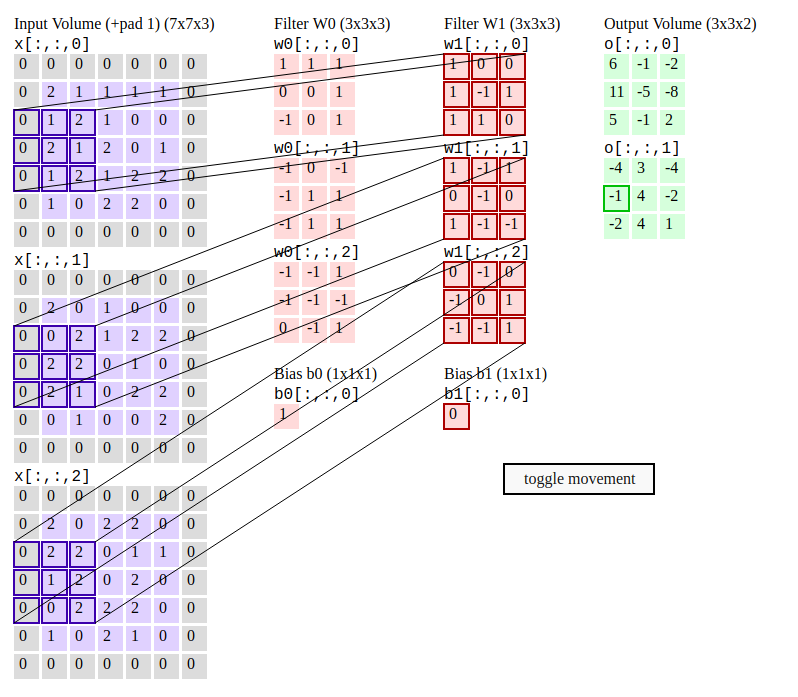
\includegraphics[width=10cm]{img/convNet.png} 
    \caption{Convolutional net with two filters \cite{SF_ConvNet} }
    \label{fig:SF_convNet}
\end{figure}

\subsubsection{Max pool layer}
Used for down-sizing the layers in-between convolutional layers. Max pool layer using the MAX operation to downsample the size, making it smaller and faster to compute the next layers. Normally the max pool filters are size 2x2, and will therefor reduze the pixel count by 75\% after the operation. The depth of the image will be the same. See the figure \ref{fig:maxpool} for more information.
\begin{figure}%
    \centering
        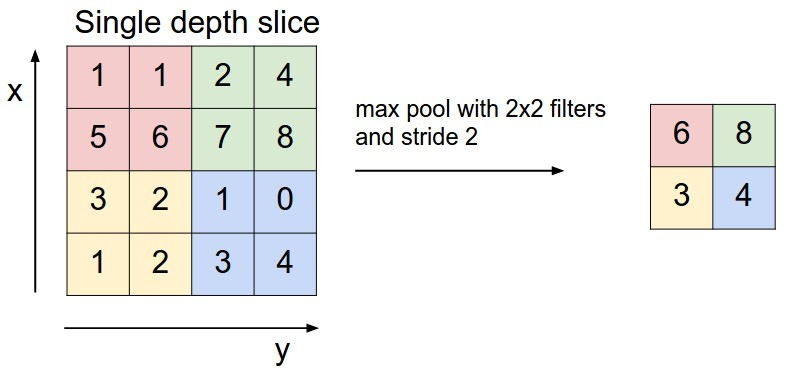
\includegraphics[width=10cm]{img/maxpool.jpeg}
    \caption{Max pool operation \cite{SF_ConvNet} }
    \label{fig:maxpool}
\end{figure}

\subsubsection{Fully Connective layer}
The fully connective layer have connections to all previous layers and is normally at the end of the "hidden layer", right before the output layer. This fully connective layer will calculate the probability of what different object are in specific position in that image with a bias. This is done by looking up highlighted areas produced by matching the highlighted areas from the convolutional filters with an activation map provided by the weight and training. 

\subsection{Training and Weights}

In order to get the convolutional layers to get their activation map, they need training. The training is done by letting the convolutional neural network process many images, maybe up to tousands of images for each object it should recognise. This recogintion phase is often done by a process called "Backpropogation". The backpropogation is done by feeding the CNN images with tags, so the network will learn to recognise key parts of different objects. A key part could be the ears of a cat. By providing enough of those images the filters will learn how to recognise different key object, who is a known feature to a specific object.

How many training images is needed depends on how well the accuracy is. However a complex weight will also demand more computations, who result in more time to process each image. There is many factors involving in how efficient the object recognition process is, but a proper sized and well trained weight is important.

Often is the weight trained on predefined imagebanks who is available online. For instance some of the YOLO weights who are published, are build on the Common Objects in COntext (COCO), image bank who is available online \cite{darknet13}.

\subsection{Intro to YOLO}\label{yolo_intro}
YOLO is an algorithm who utilises convolution neural networks (CNN) to detect object in image or video. As other approaches on image detecting with CNN like the R-CNN algorithm, they first create potential bounding boxes in the image for then to run a classifier on those boxes. After the classifier has run, post-processing remove the duplicated detections and re-trim the boundingboxes and calculate new probabilities on those boxes. 

[ref: R. Girshick, J. Donahue, T. Darrell, and J. Malik. Rich feature
hierarchies for accurate object detection and semantic
segmentation. In Computer Vision and Pattern Recognition
(CVPR), 2014 IEEE Conference on, pages 580–587. IEEE,
2014. 1, 4, 7 ]

During the traditional R-CNN algorithm, the image is run trough several times and each different component need to me trained separately. This takes a lot of time and computations. It is quite accurate, but on the cost of time. In the YOLO algorithm it is done by a single regression problem, and create the bounding boxes, probabilities and coordinates directly from the image. In order to do this task, the algorithm only iterate one time trough the image, or "You Only Look Once". The rest of the chapter will go more into details on how it is done.

\subsection{Performance}
Since YOLO only goes trough the image once, it has a potential to be quite fast. In order to utilise the performance, two different steps are essential. During compilation time, YOLO is set to choose where to be processed, GPU or CPU, and witch weight is chosen.

For comparison, a decent CPU uses about 10 seconds to render one image with a lightweight weight. Using the same weight, a high end consumer GPU have to ability to render 150 frames per seconds. 
\subsubsection*{Hardware - GPU and CPU Rendering}
With the lightest weight and on a Nvidia Titan X GPU, performance can hit about 150 frames per second, or FPS. In order to do so it is necessary to be an Nvidia GPU with CUDA capabilities. A non CUDA GPU is not supported. Why it run so fast and only featured with CUDA is because the framework of "Darknet" the backbone of YOLO is written in CUDA using "TensorFlow". TensorFlow is a framework for creating CNN and Artificial Neural Networks (ANN). The slower option is to use a CPU to process the images. This option is quite slow, but a decent CPU would be able to render an image in about 10 seconds. An older laptop CPU would render one image in about 75 seconds. 

Correct hardware is by other means quite essential for a usable real-time algorithm. 
\subsubsection*{Network Design}
When the convolutional network was designed, it was designed to pass the Pascal VOC detection dataset [9yolo] as good as possible. The architecture with GoogLeNet model for image classification as inspiration, according to the developer J. Redmon. There are designed two YOLO CNN, a normal one with 24 convolutional layers and 2 fully connected layers and the Fast YOLO. The last one uses only 9 convolutional layers \cite{YOLO}. For more information see figure \ref{fig:yolo_Convnet}.

\begin{figure}
    \centering
        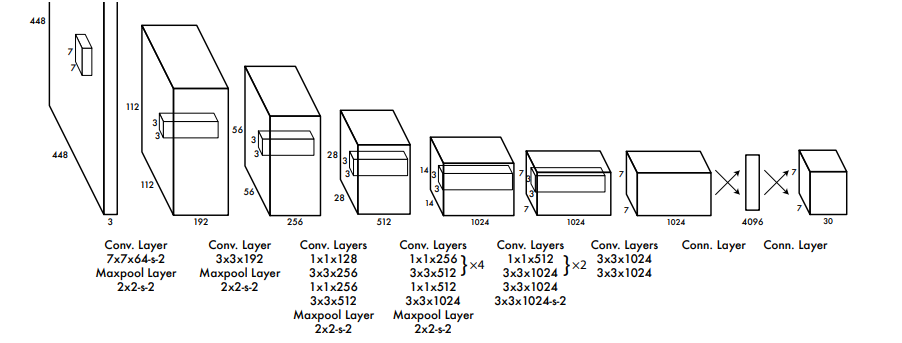
\includegraphics[width=10cm]{img/yolo_CONVnet.png}
    \caption{The CNN architecture used in YOLOv1 \cite{YOLO} }
    \label{fig:yolo_Convnet}
\end{figure}

\subsection{Why is YOLO faster?}
Like mentioned in section \ref{yolo_intro} the YOLO algorithm only look once tough the image. When YOLO take an input image, it resizes the image to for instance 416x416 pixels, and create a grid consisting of 13x13 squares. (The actual pixel size variates in the different versions of YOLO.) In each of those squares YOLO create 5 bounding boxes and calculate the probability of what object is in those bounding boxes \cite{YOLOv2}. After creating the bounding boxes, the boxes probability of containing an object is computed. All boxes giving back a probability parameter below a set threshold value is being discarded. After this process, the bounding boxes covering the same object is being connected, forming one bounding box per object, ideally. 